\pdfminorversion=4
\documentclass{beamer}
\usepackage[size=custom,width=121.92,height=91.44,scale=1.4]{beamerposter}
\usetheme{UWMadison}
\usepackage[utf8]{inputenc}
\usepackage{graphicx}
\usepackage{tikz}
\usetikzlibrary{calc}
\usepackage[style=phys]{biblatex}
\addbibresource{citations.bib}
\setbeamertemplate{bibliography item}{\insertbiblabel}
\renewcommand*{\bibfont}{\footnotesize}
\setlength{\parskip}{\baselineskip}

\title[small title]{\texorpdfstring{Statistical Methods for Pre-detonation Nuclear Forensics Analysis}
{Statistical Methods for Pre-detonation Nuclear Forensics Analysis}}
\author{Arrielle C Opotowsky, Prof. Paul PH Wilson}
\institute{University of Wisconsin-Madison}
% \date{\today}

\logo{
\includegraphics[height=8cm]{logos/cnerg.png}} % can replace with any other logo (such as DOE, NNSA, etc)
\auspice{ }

\begin{document}
\small

\begin{frame}[t]{}
%\vskip -1cm
\begin{columns}

%%%%%%%%%%%%%%%%%%%%%%%%%%%%%%%%%%%%%%%%%%%%%%%%%%%%%%%%%%%%%%%%%%%%%%%%%%%%%%%%%%%%%%%%%%%%%%%%%%%
\begin{column}[T]{0.27\textwidth}
\begin{block}{Motivation: Speeding up nuclear emergency response}

After a nuclear weapon is detonated or nuclear material is intercepted, a
priority for emergency responders is to determine both where it came from and
the radioactive danger to the public. \\~\\

While the latter can be determined
quickly, the former often involves lab work that can take days or weeks.

Presented here is a methodology that seeks to rapidly provide
investigation-guiding information using measurements taken in the field
compared against statistical models. While this work focuses on spent nuclear
fuel (SNF) from reactors outside of regulatory control, this methodology can
apply to any nuclear material, intact or remnants of a detonation. 
Statistical methods may be able to determine reactor operation parameters
faster than the traditionally utilized empirical relationships. To evaluate
their utility in this context, a number of questions must be answered.

Figure \ref{fig:itdb} blah blah.

\begin{figure}
  \fboxsep=1mm
  \fboxrule=3pt
  \fbox{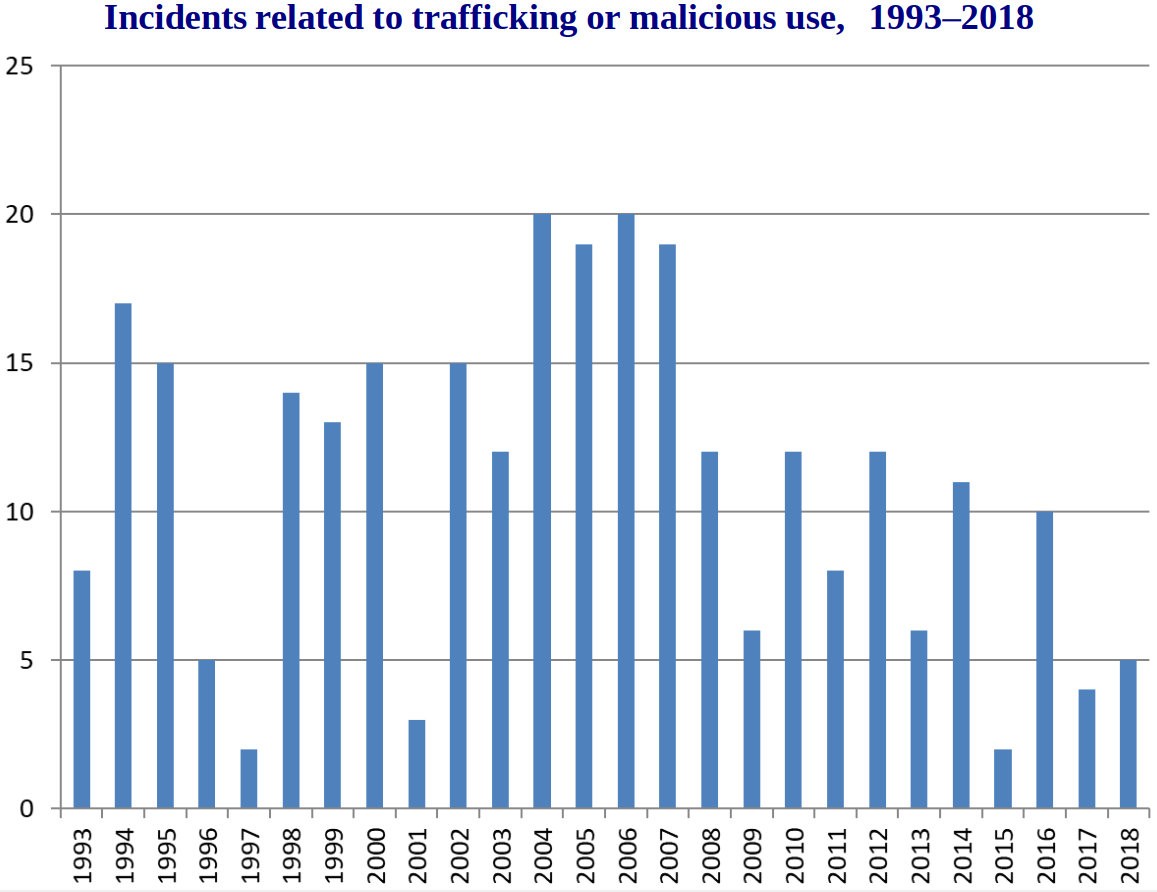
\includegraphics[height=10cm]{figures/trafficking.png}}
  \caption{138 participating countries report intercepted nuclear materials
           intended for illicit use to the IAEA.\cite{trafficking}}
  \label{fig:itdb}
\end{figure}

\end{block}

\begin{block}{Background: Using statistical methods to evaluate nuclear forensics signatures}

Nuclear forensics research initiatives include characterization of both pre-
and post-detonation materials. Measuring isotopic ratios, chemical compounds,
and trace elements are signatures used to identify the chain of custody of
these materials. One such material is spent nuclear fuel (SNF) from power
reactors. The analysis of this is usually focused on determining a set of
reactor parameters that generated the material: reactor type, fuel enrichment,
burnup, and cooling time. This provides information that can lead to the source
of the material in question.

Figure \ref{fig:ml-intro} is blah blah blah

\begin{figure}
  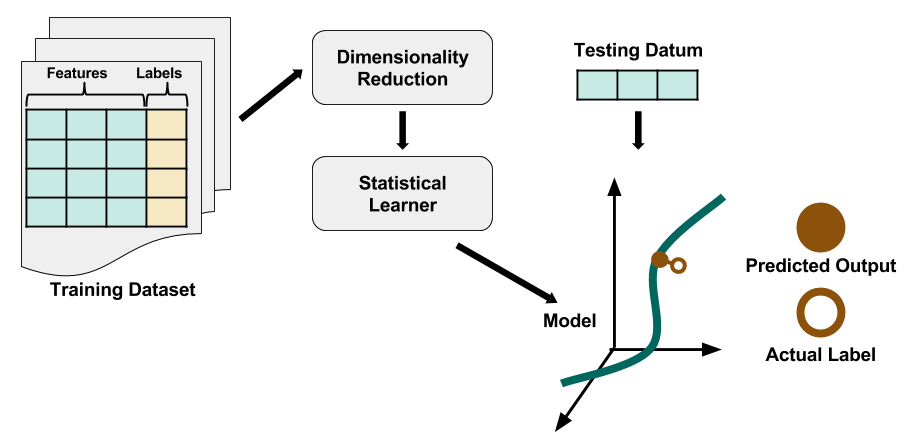
\includegraphics[width=0.8\textwidth]{figures/SupervisedRegression.png}
  \caption{Caption me}
  \label{fig:ml-intro}
\end{figure}

\end{block}
\end{column}
%%%%%%%%%%%%%%%%%%%%%%%%%%%%%%%%%%%%%%%%%%%%%%%%%%%%%%%%%%%%%%%%%%%%%%%%%%%%%%%%%%%%%%%%%%%%%%%%%%%

%%%%%%%%%%%%%%%%%%%%%%%%%%%%%%%%%%%%%%%%%%%%%%%%%%%%%%%%%%%%%%%%%%%%%%%%%%%%%%%%%%%%%%%%%%%%%%%%%%%
\begin{column}[T]{0.72\textwidth}
\begin{columns}[t]
\begin{column}{0.32\textwidth}
\begin{block}{Methodology: Maximum likelihood estimation for prediction}

Toy training set for demonstration, describe features chosen + labels of interest
Show generic ML workflow
MLE method chosen for measure of uncertainty 
Include uncertainty? 

Figure \ref{fig:overview} is blah blah blah

\begin{figure}
  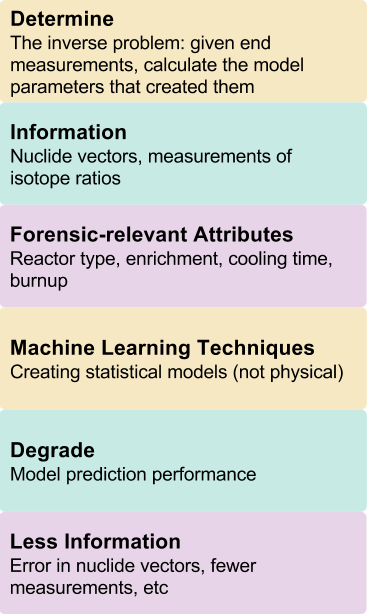
\includegraphics[height=20cm]{figures/overview.png}
  \caption{Caption me}
  \label{fig:overview}
\end{figure}

\end{block}
\end{column}

\begin{column}{0.42\textwidth}
\begin{block}{Title1}

Text1

\end{block}
\end{column}

\begin{column}{0.24\textwidth}
\begin{block}{Title2}

Text2

\end{block}
\end{column}
\end{columns}
%%%%%%%%%%%%%%%%%%%%%%%%%%%%%%%%%%%%%%%%%%%%%%%%%%%%%%%%%%%%%%%%%%%%%%%%%%%%%%%%%%%%%%%%%%%%%%%%%%%

%%%%%%%%%%%%%%%%%%%%%%%%%%%%%%%%%%%%%%%%%%%%%%%%%%%%%%%%%%%%%%%%%%%%%%%%%%%%%%%%%%%%%%%%%%%%%%%%%%%
\begin{columns}[t]
\begin{column}{0.6\textwidth}
\begin{block}{Title3}

Text3

\end{block}
\end{column}

\begin{column}{0.4\textwidth}
\begin{block}{\large References}
\printbibliography
\end{block}

\begin{block}{\large Funding}

This material is based upon work supported by the U.S. Department of Homeland
Security under Grant Award Number, 2012- DN-130-NF0001. The views and
conclusions contained in this document are those of the authors and should not
be interpreted as representing the official policies, either expressed or
implied, of the U.S. Department of Homeland Security. This material is also
based upon work supported by the U.S. National Science Foundation Graduate
Fellowship Program.

\begin{figure}
\begin{minipage}{.5\textwidth}
  \centering
  
\includegraphics[height=7.6cm]{logos/dhs.png}
\end{minipage}%
\begin{minipage}{.5\textwidth}
  \centering
  
\includegraphics[height=8cm]{logos/nsf.png}
\end{minipage}
\end{figure}

\end{block}

\end{column}
\end{columns}
\end{column}
\end{columns}
%%%%%%%%%%%%%%%%%%%%%%%%%%%%%%%%%%%%%%%%%%%%%%%%%%%%%%%%%%%%%%%%%%%%%%%%%%%%%%%%%%%%%%%%%%%%%%%%%%%
\end{frame}
\end{document}
